\section{About Monetary Economics}

Does an unanticipated shock to money affect real side of the
economy (quantities)?

\begin{itemize}
    \item CLassical view: If prices are flexible, the shock
    will change wages and prices proportionally, but not change the quantities.

    If the gov prints money and spend it, the prices increase and nominal assets lose in value, 
    which is negative wealth effect.

    Money supply increase acts like a tax on nominal asset 
    holdings, some call it 'inflation tax'.

    \item Keynesian view: Prices are rigid, so the shock will
    give a positive wealth effect, this assumes that new money is distributed proportionally to existing money holdings.
\end{itemize}

How should we conduct monetary policy?

\begin{itemize}
    \item Monetatists: steady money supply growth, in line with money
    demand growth.
    \item Keynesians: use expansionary MP to stimulate the economy
    in a recession.
    \item Inflation of 70's and subsequent successful tight MP(Volcker)
    led to Monetarists becoming very influential.
\end{itemize}

\textcolor{blue}{Problems of previous models}

\begin{itemize}
    \item Old models are subject to the Lucas critique(policy changes
    may affect people's response to the policies)
    \item Hard to take seriously from a quantitative perspective
\end{itemize}

Since RBC model has try to use dynamic method to explain the economy, 
people start putting money into the model.

\begin{itemize}
    \item Outcome from this program is the “New Keynesian
    Synthesis”: combine RBC models with price rigidities.
    \item Money is non-neutral in the short run (Keynesian
    element), and neutral in the long run (classical element).
\end{itemize}

\section{The Monetary Transmission Mechanism}

\subsection{Households and nominal assets}

Nominal assets are bonds $B_t$ which pay interest at nominal rate $i_t$.
Ignore the labor-leisure choice, the households maximize:
\begin{align*}
    \max & \quad \mathbb{E}_t \sum_{i=0}^{\infty}U(C_{t+i} )\\
    \text{s.t.} & \quad P_{t+i}C_{t+i} + P_{t+i}K_{t+i+1} + B_{t+i+1} = W_{t+i}L + P_{t+i}(1+r_{t+i})K_{t+i} + (1+i_{t+i})B_{t+i} 
\end{align*}
where $W$ is the nominal wage, $P$ is the price of cunsumption goods,
$r_{t+i}$ is the rental rate of capital net of depreciation.

Define the Lagrangian:
\begin{align*}
    \mathcal{L} = \mathbb{E}_t\sum_{i=0}^{\infty} \left[ U(C_{t+i} ) + \lambda_{t+i} \left( W_{t+i}L + P_{t+i}(1+r_{t+i})K_{t+i} + (1+i_{t+i})B_{t+i} - P_{t+i}C_{t+i} - P_{t+i}K_{t+i+1} - B_{t+i+1} \right) \right]
\end{align*}

The FOCs are:
\begin{align*}
    U^{\prime} (C_{t+i} ) &= \mathbb{E}_t P_{t+i}\lambda_{t+i}  \\
    P_{t+i}\lambda_{t+i} &= \mathbb{E}_t \lambda_{t+i+1} P_{t+i+1} (1+r_{t+i+1}) \\
    \lambda_{t+i} &= \mathbb{E}_t \lambda_{t+i+1} (1+r_{t+i+1}) \\
\end{align*}
Combining the first two, we get the standard Euler equation:
\[
    U^{\prime} (C_{t} ) = \mathbb{E}_t \left(U^{\prime} (C_{t+1} ) (1+r_{t+1})\right)
\]
Conbine the first and the third:
\[
    U^{\prime} (C_{t} ) = \mathbb{E}_t \left(\frac{1+i_{t+1}}{1+\pi_{t+1}} U^{\prime} (C_{t+1} )\right)
\]
where inflation $\pi = \frac{P_{t+1} - P_t}{P_t}$.

\begin{align*}
    U^{\prime} (C_{t} ) &= \mathbb{E}_t \left(\frac{1+i_{t+1}}{1+\pi_{t+1}} U^{\prime} (C_{t+1} )\right) \\\\
    U^{\prime} (C_{t} ) &= \mathbb{E}_t \left((1+r_{t+1}) U^{\prime} (C_{t+1} )\right) \\\\
\end{align*}

\begin{itemize}
    \item What matters for the intertemporal consumption decision is
    the real interest rate, not the nominal interest rate.
    \item The FOC are necessary conditions for having both positive $B$
    and positive $K$. By the two equations above, we get:
    \[1+r_{t+1} = \frac{1+i_{t+1}}{1+\pi_{t+1}}. \]
    So, the \textcolor{red}{real return(interest rate)} of a nominal asset
    with \textcolor{red}{nominal interest rate} $1+i_{t+1} $ is: $\frac{1+i_{t+1} }{1+\pi_{t+1}}$.
    % \item This is the Fisher equation.
\end{itemize}

\begin{corollary}[Fisher equation]
    \ 

    It's the relationship between asset returns that has to hold 
    so that the household is willing to hold positive amounts 
    of these assets in their portfolio (or: if you allow negative 
    holdings, to clear asset markets). \\
    When households are risk-neutral, the FOCs become:
    \[\mathbb{E}_t (1+r_{t+1}) = \mathbb{E}_t \left(\frac{1+i_{t+1}}{1+\pi_{t+1}}\right) \]
    In a deterministic world, there's no $E$, which is often approxima
\end{corollary}

\subsection{Firms}
The firms would like to maximize profits, with perfect competition adn frictionless factor markets:
\[MPK = r\]
Again, real interest rate matters. 

\textbf{Conclusion:} if monetary policy should affect demand, the real interest rate is the key price in the economy.

\section{The tools of monetary policy}
So, in order to stimulate demand, the central bank needs to change the real interest rate.

\subsection*{How?}

\begin{itemize}
    \item Change the money supply, with demand curve, this would implement a particular nominal interest rate.
    \item Change the nominal interest rate directly.
\end{itemize}

\begin{tikzpicture}[
    node distance=1.5cm,
    block/.style={
        rectangle,
        draw,
        fill=blue!20,
        text width=5cm,
        text centered,
        rounded corners,
        minimum height=1cm
    },
    arrow/.style={
        thick,
        ->,
        >=Stealth
    }
]

% Nodes
\node (centralbank) [block] {Central Bank};

% First branch
\node (nominalrate1) [block, below left=of centralbank, xshift=2cm, yshift=-1cm] {Nominal interest rate i};

% Second branch
\node (nominalrate2) [block, below right=of centralbank, xshift=-2cm, yshift=-1cm] {Nominal interest rate i};

% Combined branch
\node (realrate) [block, below=of centralbank, yshift=-3cm] {Real interest rate r};
\node (consumption) [block, below=of realrate] {Consumption, Investment};
\node (output) [block, below=of consumption] {Output};

% Arrows for the first branch
\draw [arrow] (centralbank) -- (nominalrate1) node[midway, left, text width=3cm, align=left] {Sets and implements interest rate target};
\draw [arrow] (nominalrate1) -- (realrate) node[midway, left] {Nominal rigidities (?)};

% Arrows for the second branch
\draw [arrow] (centralbank) -- (nominalrate2) node[midway, right, text width=3cm, align=left] {Sets money supply, given a money demand curve and money market clearing we get a nominal interest rate i};
\draw [arrow] (nominalrate2) -- (realrate) node[midway, right] {Nominal rigidities (?)};

% Arrows for the combined branch
\draw [arrow] (realrate) -- (consumption) node[midway, left] {Intertemporal Euler equation};
\draw [arrow] (consumption) -- (output) node[midway, left] {Given an output supply curve};

\end{tikzpicture}

\subsection*{Money supply-demand equilibrium}

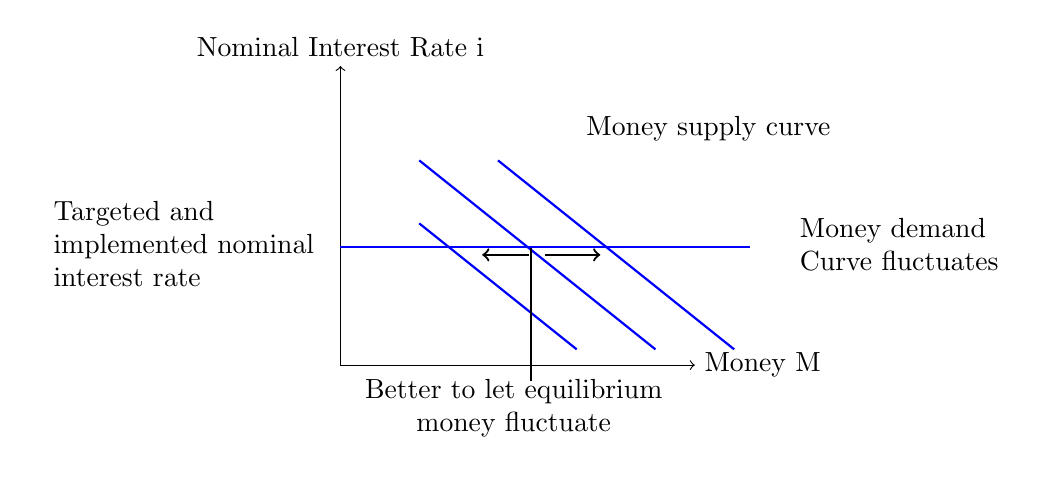
\begin{tikzpicture}[scale=1]
    \draw[->] (0,0) -- (4.5,0) node[right] {Money M};
    \draw[->] (0,0) -- (0,3.8) node[above] {Nominal Interest Rate i};
    
    % Money demand curves
    \draw[blue, thick] (1,2.6) -- (4,0.2);
    \draw[blue, thick] (2,2.6) -- (5,0.2);
    \draw[blue, thick] (1,1.8) -- (3,0.2);
    
    % % Money supply curve (vertical line)
    \draw[black, thick] (2.42,1.5) -- (2.42,-0.2);
    
    % Horizontal line for targeted interest rate
    \draw[blue, thick] (0,1.5) -- (5.2,1.5);
    
    % Arrows showing fluctuation
    \draw[->, thick] (2.4,1.4) -- (1.8,1.4);
    \draw[->, thick] (2.6,1.4) -- (3.3,1.4);
    
    % Labels
    \node[left] at (0,1.5) {\begin{tabular}{l}Targeted and\\implemented nominal\\interest rate\end{tabular}};
    \node[below] at (2.2,0) {\begin{tabular}{c}Better to let equilibrium\\money fluctuate\end{tabular}};
    \node[right] at (3,3) {Money supply curve};
    \node[right] at (5.5,1.5) {\begin{tabular}{l}Money demand\\Curve fluctuates\end{tabular}};
\end{tikzpicture}

\section{A model of the interbank market}
\begin{itemize}
    \item Market participants: $n$ banks.
    \item Banks hold reserves at the central bank.
    \item REserves are used for settling transfers between banks arising from the payment system.
    \item Banks are unsure of the transfers htey will need to make.
    \item Banks can borrow reserves from one another in the interbank market,
    but do not know how much reserve they'll require at the point they participate in the interbank market.
    \item Banks can also acquire reserves through the repo (repurchase
    agreement) market. The central bank can be a participant in
    this market.
\end{itemize}

\begin{note}
    \ 

    $B_j$ = reserves of bank $j$ at beginning-of-period.(after previous debts settles) \\
    $I_j$ = net borrowing in the interbank market (negative for
    lending) by bank $j$. \\
    $P_j$ = net bond repos(sales and repurchases) by bank $j$. \\
    $T_j$ = net payment bank $j$ make to other banks. \\
    $R_j$ = balance of bank $j$ at end-of-period. \\
    Accounting: $R_j = B_j + I_j + P_j - T_j$.
\end{note}

\subsection{Interbank market and repo market}
\textbf{Interbank market:}
\begin{itemize}
    \item Uncollateralized loans between banks.(银行间无抵押贷款, potentially risky)
    \item Interest rate $i$.
\end{itemize}

\textbf{Repo market:}
\begin{itemize}
    \item Sell bond now and agree to repurchase later.
    \item Effectively a collaboratized loan, so risk-free if collateral is good.
\end{itemize}

\begin{note}[Central bank facilities]
    \ 

    \textbf{Deposit Facility:} Centrla bank offers an interest rate of $i_d$ on deposit balances in banks' account at the end of time period.

    \textbf{Borrowing facility:} Central bank charges an interest rate $i_b$ on negative balances in banks' accounts.
    \begin{itemize}
        \item Positive spread over deposit rate: $i_b > i_d$.
        \item Equivalent to an offer to make loans at the end of perios, with the oad credited to the bank's account.
        \item Collateral required -- we should assune banks have enough collateral to use it.
    \end{itemize}
\end{note}

\subsection{Balance on account next period}

Reserve balance of bank $j$ at the end of period is:
\[
B^{\prime} _j = R_j - (1+i)(I_j + P_j) + \left\{\begin{matrix}
   i_d R_j & \text{if } R_j \geq 0\\
   i_b R_j & \text{if } R_j < 0
  \end{matrix}\right.
\]
Since $R_j = B_j + I_j + P_j - T_j$, we have:
\[
B^{\prime} _j = B_j - T_j - i(I_j + P_j) + \left\{\begin{matrix}
   i_d (B_j + I_j + P_j - T_j) & \text{if } B_j + I_j + P_j - T_j \geq 0\\
   i_b (B_j + I_j + P_j - T_j) & \text{if } B_j + I_j + P_j - T_j < 0
  \end{matrix}\right.
\]

Assume banks are risk-neutrala, and they aim to maximize their next period expected balance $\mathbb{E}(B^{\prime}_j)$.
Choice variabls are: interbank transaction $I_j$, repo market transaction $P_j$.
\begin{align*}
    \mathbb{E}(B^{\prime}_j) = B_j - i(I_j + P_j) &+ i_d \int_{-\infty}^{B_j + I_j + P_j} (B_j + I_j + P_j - T_j) dF(T_j) \\
    &+ i_b \int_{B_j + I_j + P_j}^{\infty} (B_j + I_j + P_j - T_j) dF(T_j)
\end{align*}
The FOCs are:
\begin{align*}
    \frac{\partial \mathbb{E}(B^{\prime}_j)}{\partial I_j} &= 0 \\
    \frac{\partial \mathbb{E}(B^{\prime}_j)}{\partial P_j} &= 0
\end{align*}

Two equations lead to the same equation, so we only consider one of them.
\begin{theorem}[Leibniz Rule]
    \ 
    
    Let $f(x, t)$ be a function such that both $f(x, t)$ and 
    its partial derivative $f_x(x, t)$ are continuous in $t$ and 
    $x$ in some region of the $xt$-plane, 
    including $a(x) \leq t \leq b(x)$, $x_0 \leq x \leq x_1$. 
    Also suppose that the functions $a(x)$ and $b(x)$ are both continuous 
    and both have continuous derivatives for $x_0 \leq x \leq x_1$. 
    Then, for $x_0 \leq x \leq x_1$,
    \[
    \frac{d}{dx} \left( \int_{a(x)}^{b(x)} f(x, t) \, dt \right) = f(x, b(x)) \cdot \frac{d}{dx} b(x) - f(x, a(x)) \cdot \frac{d}{dx} a(x) + \int_{a(x)}^{b(x)} \frac{\partial}{\partial x} f(x, t) \, dt.
    \]
\end{theorem}

Use the Leibniz rule:
\begin{align*}
    & \frac{\partial}{\partial I_j} \int_{-\infty}^{B_j + I_j + P_j} (B_j + I_j + P_j - T_j) dF(T_j) \\
    &= \int_{-\infty}^{B_j + I_j + P_j} f(T_j)d T_j + \left((B_j + I_j + P_j) - (B_j + I_j + P_j)\right)f(B_j + I_j + P_j) \\
    &= F(B_j + I_j + P_j) 
\end{align*}
Similarly,
\begin{align*}
    & \frac{\partial}{\partial I_j} \int_{B_j + I_j + P_j}^{\infty} (B_j + I_j + P_j - T_j) dF(T_j) \\
    &= 1 - F(B_j + I_j + P_j)
\end{align*}
Hence, the FOC reduces to:
\[
-i + i_d F(B_j + I_j + P_j) + i_b (1 - F(B_j + I_j + P_j)) = 0
\]
Equivalently,
\[
(i - i_d)F(B_j + I_j + P_j) = (i_b - i)(1 - F(B_j + I_j + P_j))
\]
The optimal demand for interbank and repo lending is characterized by the equation: 
\[
F(B_j + I_j + P_j) = \frac{i_b - i}{i_b - i_d}
\]

\subsection{Aggregation and market clearing}
\begin{align*}
    B &= \sum_{j=1}^{n}B_j (\text{Aggregate beginning-of-period balances})\\
    P &= \sum_{j=1}^{n}P_j (\text{Aggregate end-of-period balances})\\
    T &= \sum_{j=1}^{n}T_j = 0 (\text{payments between banks cancel out})  \\
    R &= \sum_{j=1}^{n}R_j
\end{align*}

Since $R_j = B_j + I_j + P_j - T_j$, we have $R = B+P$ in the aggregate.

Since $B_j + I_j + P_j$ is the same for all banks: $B_j + I_j + P_j = \frac{R}{n}$.

\subsection{Equilibrium interbank interest rate}
\begin{align*}
    F\left(\frac{R}{n}\right) &= \frac{i_b - i}{i_b - i_d} \\
    \frac{R}{n} &= F^{-1}\left(\frac{i_b - i}{i_b - i_d}\right) \\
    i &= i_d + \frac{i_b - i_d}{n} \int_{-\infty}^{F^{-1}\left(\frac{i_b - i}{i_b - i_d}\right)} x dF(x)
\end{align*}

THe central bank directly controls:
\begin{itemize}
    \item $i_d$ and $i_b$.
    \item Open market operations $P$.
\end{itemize}
Indirectly determinems
\begin{itemize}
    \item Interbank and repo rate $i$.
    \item Total end-of-period reserves $R = B+P$.
\end{itemize}

\subsection{Interbank market with channel system}
\begin{itemize}
    \item \textbf{Demand:} Equation $F\left(\frac{R}{n}\right) = \frac{i_b - i}{i_{b-i_d}}$, giving a negative relationship between $i$ and $R$.
    \item \textbf{Supply:} Central bank sets $R = B+P$ by open market operations.
\end{itemize}

If we hold all other policy instruments constant,
\begin{itemize}
    \item An increase in total reserves $R$ will shift supply curve to the right, decreasing $i$.
    \item An increase in $i_d$ will shift demand curve upward, increasing $i$.
    \item An increase in $i_b$ will shift demand curve upward, increasing $i$.
\end{itemize}

\begin{note}
    \ 

    A narrow channel has advantages:
    \begin{itemize}
        \item More precise control of $i$, less fluctuations.
        \item Less need for open market operations.
    \end{itemize}

    There'are also disadvantages, e.g. $i_b = i_b$:
    \begin{itemize}
        \item Trading in interbank market dries up.
        \item CB becomes the intermediary of all borrowing and lending between banks, hence it incurs the cost of monitoring credit-worthiness of banks. \textcolor{red}{It's not the central bank's job.}
    \end{itemize}
\end{note}

\subsection{Interest rate maturity}

\begin{question}
    How does this affect medium- and long-term interest rates? How are interest rates of different maturities related?
\end{question}

\begin{eg}
    \ 

    Imagine an investor invest for 2 years:
    \begin{itemize}
        \item Buy a 2-year bond, keep until it matures: \[\text{return} = 1 + i_t^{(2y)}\]
        \item Buy a 1-year bond, then buy another 1-year bond: \[\text{return} = (1+i_t^{(1y)})(1+i_{t+1}^{1y})\]    
    \end{itemize}

    \textbf{Expectations Hypothesis:} Expectations of these two returns should be the same:
    \[i_t^{(2y)} = \mathbb{E}_t (1 + i_t^{(1y)})(1 + i_{t+1}^{(1y)}).\]

    This should hold exactly if agents are risk-neutral. WIth risk aversion, one would adjust the expected retuen for riskiness.
\end{eg}
